\documentclass{article}[11pt]
\textheight 8.5in
\usepackage{graphicx}
\usepackage{float}%for forcing position of figs
\usepackage{hyperref}
\usepackage{amsmath}
\usepackage{amssymb}

\begin{document}
\begin{center}
Siddharthan Rajasekaran\\
Week of 3/20/2017 - 3/27/2017
\end{center}

\section{Summary of Discussions}
In this report, we will talk about the initial implementation of GPIRL. We will compare the results of GPIRL to that of MaxEnt IRL \cite{ziebart2010modeling} in case of nonlinear reward function. We will be using the exact same example shown in the GPIRL paper \cite{levine2011nonlinear}

\section{Object world}
We consider an object world (which is just a grid world with objects placed an certain positions) for our evaluation. Each object has an outer and inner color. The feature vector is taken as the nearest euclidean distance to every possible outer and inner colored object. We use a palette of $\mathcal{C}$ colors and hence have a feature vector of size $2 \times |\mathcal{C}|$ corresponding to nearest object with a specific inner or outer color. The true reward is is +1 in states that are both within 3 units from blue outer color and within 2 units from red outer color, -1 within 3 units from blue outer color, 0 otherwise. Note that the reward is non-linear in the feature vector, that is, it cannot be expressed as a weighted combination of each dimension in feature vector. This is the reason MaxEnt-IRL may find it difficult (it actually does!) to express the reward and optimize over the weights. 



\begin{figure}[H]
  \begin{center}
    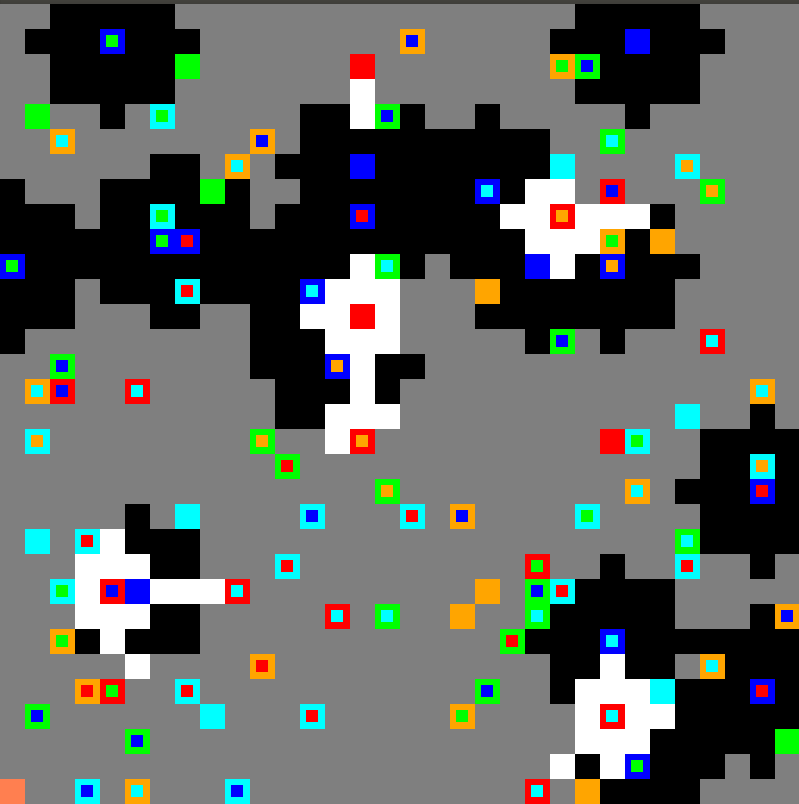
\includegraphics[width=1\linewidth]{images/32grid}
    \caption{Object world showing randomly place objects. Each object has an outer and inner color. The reward is +1 in states that are both within 3 units from blue outer color and within 2 units from red outer color, -1 within 3 cells from blue outer color, 0 otherwise. Note that this is non-linear in euclidean distance to each object. The feature vector is the euclidean distance to all the outer and inner colorsThe rewards are shown in grey scale -- white = +1, grey = 0, black = -1.}
    \label{fig:converge}
  \end{center}
\end{figure}


 
\section{Results of implementation}

We use the ARD kernel for the GP as in the paper. The kernel is of the form
\begin{align*}
k(x_i,x_j) = \beta \exp \Big (-\frac{1}{2}(x_i - x_j)^T \Lambda (x_i - x_j) - \textbf{1}_{i \neq j} \sigma^2 tr(\Lambda) \Big )
\end{align*}
 Once the gradient descent converges (i.e, $||gradient||_\infty < \epsilon$) , we have a reward labels for each inducing points (the feature vector evaluated at each state in demonstration) and the hyper-parameters $\Lambda$ and $\beta$. 
 
 In our implementation, we use a palette of colors $['blue', 'red', 'greean', 'cyan', 'orange']$. We perform GPIRL on a 5x5 grid as shown in Fig.ref{fig:5grid} and get the following $\Lambda$
 
\begin{align*}
\Lambda = diag([ 0.94888776,  0.6064871,   7.32826548,  7.00056063 , 0.36345795 , 7.01155729,\\
7.44337621 , 0.78492381 , 1.07347592 , 1.21262448])
\end{align*} The first five elements of $\Lambda$ correspond to the weights to be multiplied to the distance to the inner color and the last 5 correspond to that of outer color. Note that in this object world, we do not know if the rewards are due to inner or outer colors as there are only 2 objects. Hence GPIRL should learn that inner colors 'green' and 'cyan' are more relevant than other inner colors. Similarly, the same should be leaned for the outer colors 'blue' and 'red'. This is why we see a large value of lambda at inner colors green and cyan (index 3 and 4 in $\Lambda$) and at outer colors blue and red (index 6 and 7 in $\Lambda$). A high value of $\Lambda$ implies that the reward is highly affected by the corresponding features. This can also be learned by GPIRL in case of extra objects (dis-tractors) which will also help us disambiguate the importance of green and cyan (inner) from blue and red (outer). 



 \begin{figure}[H]
  \begin{center}
    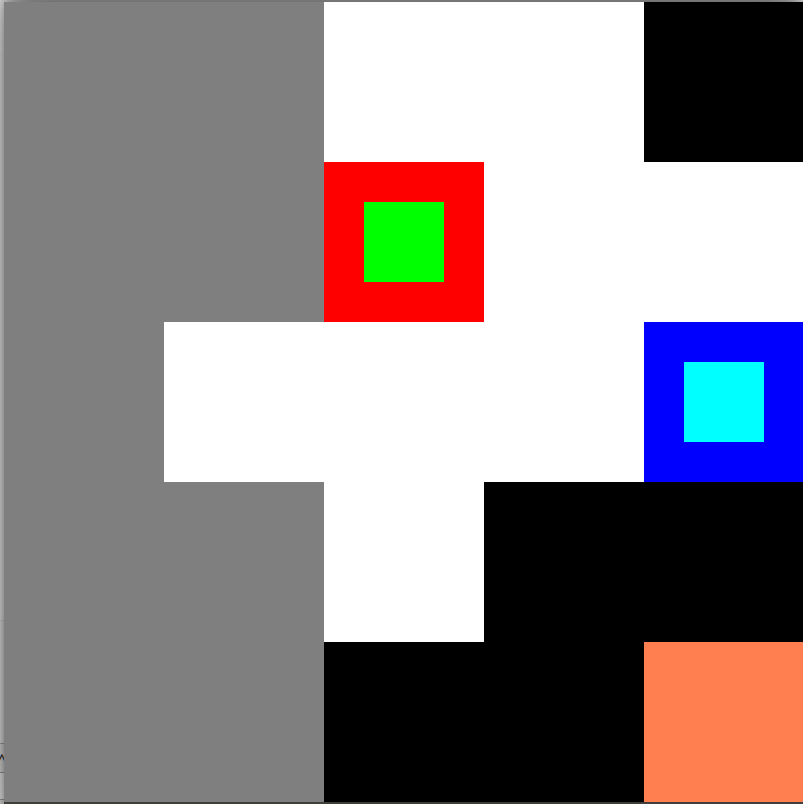
\includegraphics[width=0.8\linewidth]{images/5grid}
    \caption{5x5 test grid to compare GPIRL and MaxEnt IRL. We have two objects placed at (0,2) and (2,1). The Coral colored cell is the agent}
    \label{fig:5grid}
  \end{center}
\end{figure}


The following figures. \ref{fig:max} and \ref{fig:gpirl} show the recovered reward using MaxEnt IRL and GPIRL respectively. The GPIRL actually learns every positive reward cells with positive values and every negative with negative values. This is a remarkable difference from MaxEnt IRL. In MaxEnt IRL we are assuming a linear combination of features as reward. Note how the reward linearly varies as we move away from the top left corner. Though MaxEnt IRL can approximate the reward regions (higher reward if you go top left), GPIRL simply nails the reward values (although there is difference in exact values) including the signs for every cell. The reason why GPIRL has errors in the magnitudes is because the ARD kernel assumes a smoothly varying reward function. To represent such step reward functions, one should use the alternate kernel provided in the paper. \textbf{This work will be soon done and the results will be added to this section}. However, the main this to note is that we are able to approximate a non linear reward function much better than the MaxEnt IRL. 

Often the reward function for human action is non-linear in simple features. For example, work done is a non-linear function of joint velocities. Hence instead of worrying about exactly defining the features with which the reward can be expressed linearly, we can just give several features that matter like velocity, relative angle between the object to be grasped and the arm ...etc instead of worrying about giving sine(angle) or secant(angle) for instance



 \begin{figure}[H]
  \begin{center}
    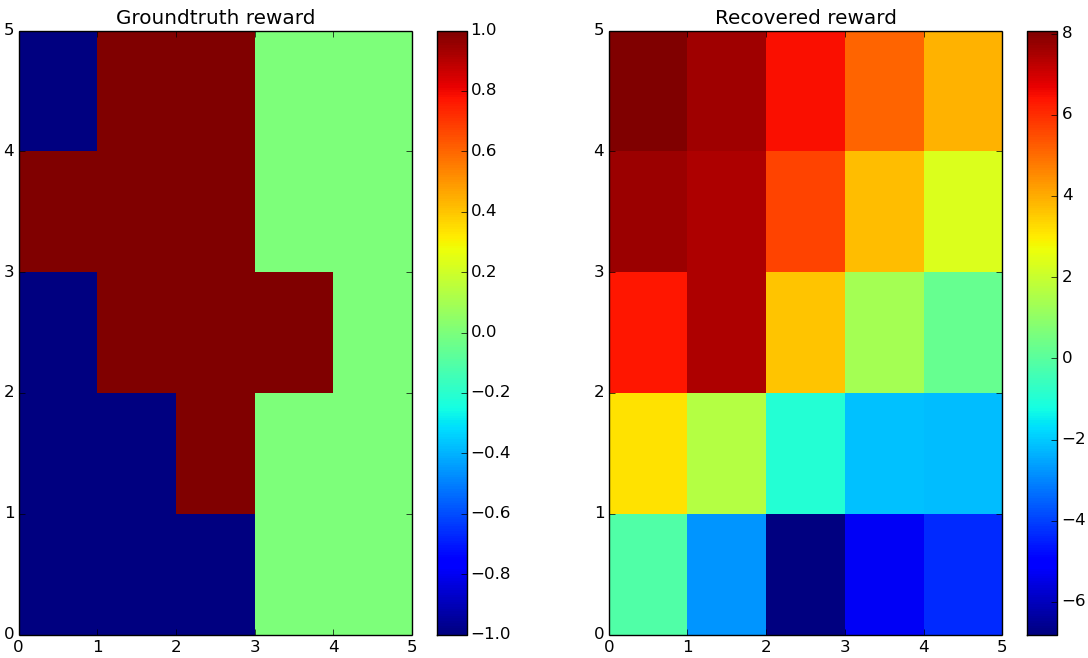
\includegraphics[width=1\linewidth]{images/maxent_results}
    \caption{True vs Recovered reward using MaxEnt IRL. \textit{Note: The colors can be misleading as the values have been re-scaled}}
    \label{fig:max}
  \end{center}
\end{figure}


 \begin{figure}[H]
  \begin{center}
    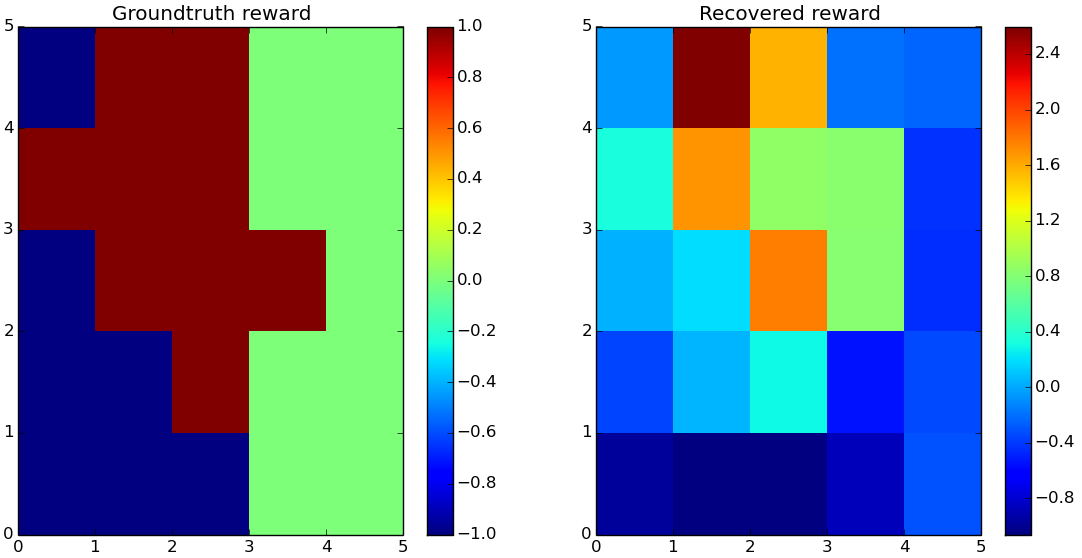
\includegraphics[width=1.07\linewidth]{images/gpirl_results}
    \caption{True vs Recovered reward using GPIRL. \textit{Note: The colors can be misleading as the values have been re-scaled}}
    \label{fig:gpirl}
  \end{center}
\end{figure}



\section{Plan for next week}
I will finish up the alternative kernels for GPIRL (in the paper) to approximate step functions (function that are not smooth).Though we gain more intuition from implementation on very small object world, I will also test the algorithm on 32x32 grid for a proof of concept. Some insights woth exploring in GPIRL: with small values of $\sigma$ in the kernel function, we get degenerate covariance matrices which means we do not have a minimalist representation of inducing points. Can we exploit this to find the linearly independent inducing points? Will a degenerate covariance matrix for a given $\sigma$ be fully ranked in the next iteration? \\

\textbf{Making it work in high dimensional systems:} The main reason MaxEnt IRL or GPIRL is slow is because of the softvalue iteration until convergence. Actually, if one can store Q values for every state action pair, then it is reasonable to use a reward function for every state action pair too. We can always generalize this function (r(s,a)) better than GPIRL offline with features and many methods in Machine Learning. So one way to make GPIRL more important is to extend it to higher dimensional state space where even the Q functions cannot have a value for every state action pair. Extending the methods to approximate Q-learning methods will be very reasonable. Also, another way to avoid value iteration is to use policy search methods. There are many cross entropy based methods and policy gradient based methods. After all, we only perform value iteration to get a policy. Recently, I was going through Trust Region Policy Optimization (TRPO) \cite{schulman2015trust} which is based on Approximately Optimal Approximate Reinforcement Learning \cite{kakade2002approximately} and I find it very interesting and promising. I believe exploring the combination of these value iteration based IRL methods with these policy search methods will be worthwhile. 

\section{Long-Term Plan}
We discuss some possible directions here. These ideas may be sketchy but can open up potential future directions. 'Making it work in high dimensional systems' (previous paragraph) is partially a long term object and should be added here in future reports
\subsection{Learning the discount factor}
Generally, in policy gradient methods, we assume a stochastic policy instead of deterministic ones. The nice thing about stochastic policies is that they smooth out the problem. In case we have a step reward function (we often do), a parametrized stochastic policy allows us to take the gradient of cumulative reward with respect to the parameters so that we can perform gradient descent to find a optimum. This is done even when we want to learn a deterministic policy. 

 \url{http://inst.eecs.berkeley.edu/~cs294-40/fa08/scribes/lecture2.pdf} gives a proof of the convergence of value iteration. We can see that the bellman backup operator is a max-norm $\gamma$ contraction (max norm distance between bell man backups of 2 values of a state is factored by $\gamma$). Changing $\gamma$ definitely is somehow related to the optimal value (and hence the optimal policy changes with $\gamma$). If we can define a stochastic optimal policy (like MaxEnt IRL) and find its gradient with respect to $\gamma$, we could inverse learn $\gamma$ using the demonstrations. This idea is sketchy, but I should explore this direction more to see if this is possible.
 
\subsection{Transfer Learning}
Traditionally transfer learning uses bisimulation metric between states from different tasks (source and target) and transfers the knowledge, for example the values of states that are close by according to this metric. Can we extend this idea to the inverse learning problem. That is, given demonstrations for two different tasks, can we learn the reward function of the second task faster by transferring some knowledge about the reward function from the first. For instance, GPIRL simply works for any randomly generated object world since it learns the actual reward function. Can we also use the new demonstrations in the target task to come up with additional mapping for a changing reward function? 




\section{Backlogs in GPIRL}
\begin{enumerate}
\item Alternative kernel
\item 32x32 Grid example
\end{enumerate}

\section{Bibliography}

\bibliographystyle{plain}
\bibliography{bibfile}
\end{document}
